\documentclass[tikz,border=4pt]{standalone}
\usepackage{amsmath,amssymb}\usepackage[scaled]{helvet}\renewcommand\familydefault{\sfdefault}
\usetikzlibrary{positioning,arrows.meta,fit,backgrounds,shapes.geometric}
\definecolor{c1}{HTML}{2F5D8A}\definecolor{c2}{HTML}{D9822B}\definecolor{c3}{HTML}{3C8D5A}\definecolor{c4}{HTML}{8A3B5D}\definecolor{g}{HTML}{F2F2F2}
\tikzset{b/.style={draw=#1,fill=#1!8,rounded corners=3pt,align=center,font=\footnotesize,minimum height=1.05cm,text width=2.75cm,line width=0.8pt},
 a/.style={-{Latex[length=2.2mm]},line width=0.8pt,draw=black!70}, lab/.style={font=\scriptsize\bfseries,text=#1}}
\begin{document}
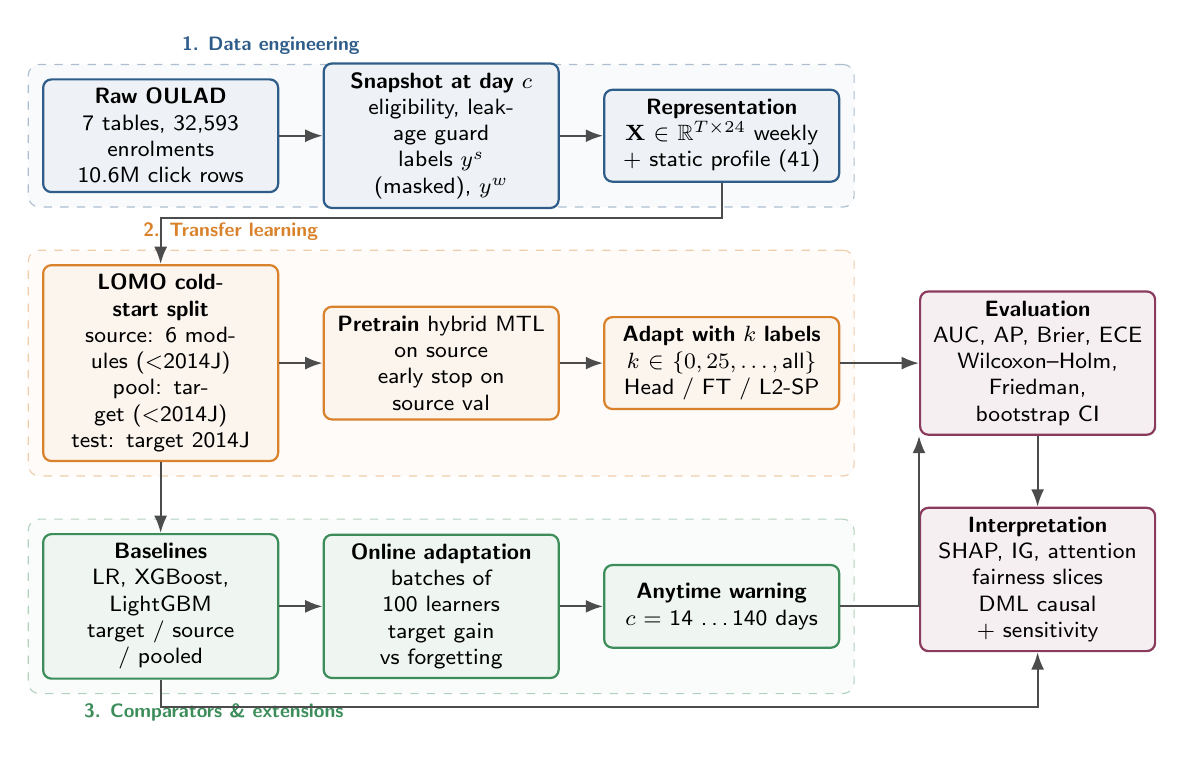
\begin{tikzpicture}[node distance=0.45cm and 0.55cm]
\node[b=c1] (raw) {\textbf{Raw OULAD}\\7 tables, 32,593 enrolments\\10.6M click rows};
\node[b=c1,right=of raw] (snap) {\textbf{Snapshot at day $c$}\\eligibility, leakage guard\\labels $y^s$ (masked), $y^w$};
\node[b=c1,right=of snap] (feat) {\textbf{Representation}\\$\mathbf{X}\in\mathbb{R}^{T\times24}$ weekly\\+ static profile (41)};
\node[b=c2,below=0.9cm of raw] (split) {\textbf{LOMO cold-start split}\\source: 6 modules ($<$2014J)\\pool: target ($<$2014J)\\test: target 2014J};
\node[b=c2,right=of split] (pre) {\textbf{Pretrain} hybrid MTL\\on source\\early stop on source val};
\node[b=c2,right=of pre] (adapt) {\textbf{Adapt with $k$ labels}\\$k\in\{0,25,\dots,\text{all}\}$\\Head / FT / L2-SP};
\node[b=c3,below=0.9cm of split] (base) {\textbf{Baselines}\\LR, XGBoost, LightGBM\\target / source / pooled};
\node[b=c3,right=of base] (stream) {\textbf{Online adaptation}\\batches of 100 learners\\target gain vs forgetting};
\node[b=c3,right=of stream] (any) {\textbf{Anytime warning}\\$c$ = 14 \dots 140 days};
\node[b=c4,right=1.0cm of adapt] (eval) {\textbf{Evaluation}\\AUC, AP, Brier, ECE\\Wilcoxon--Holm, Friedman,\\bootstrap CI};
\node[b=c4,below=0.9cm of eval] (xai) {\textbf{Interpretation}\\SHAP, IG, attention\\fairness slices\\DML causal + sensitivity};
\draw[a] (raw)--(snap); \draw[a] (snap)--(feat); \draw[a] (feat.south) |- ++(0,-0.45) -| (split.north);
\draw[a] (split)--(pre); \draw[a] (pre)--(adapt); \draw[a] (adapt)--(eval);
\draw[a] (split)--(base); \draw[a] (base.east)--(stream.west); \draw[a] (stream)--(any);
\draw[a] (any.east) -| (eval.south west); \draw[a] (base.south) |- ++(0,-0.35) -| (xai.south);
\draw[a] (eval)--(xai);
\begin{scope}[on background layer]
\node[fit=(raw)(feat),fill=c1!3,draw=c1!40,dashed,rounded corners,inner sep=5pt,label={[lab=c1]above left:1. Data engineering}] {};
\node[fit=(split)(adapt),fill=c2!3,draw=c2!40,dashed,rounded corners,inner sep=5pt,label={[lab=c2]above left:2. Transfer learning}] {};
\node[fit=(base)(any),fill=c3!3,draw=c3!40,dashed,rounded corners,inner sep=5pt,label={[lab=c3]below left:3. Comparators \& extensions}] {};
\end{scope}
\end{tikzpicture}
\end{document}
